\section{Grundlagen}
Im folgenden Kapitel werden die theoretischen Grundlagen behandelt, die für das Verständnis dieser Arbeit notwendig sind. Dabei geht es in erster Linie um allgemeine Begrifflichkeiten aus dem wirtschaftlichen Kontext des zu entwickelnen Programms.

\subsection{ERP-Systeme}
ERP ist ein Akronym für den englischen Begriff \glqq{}Enterprise Ressource Planning\grqq{}, also das Planen von Unternehmensressourcen, u.a. in den Bereichen Beschaffung, Produktion, Vertrieb, Personalwirtschaft und Finanzwesen. \footcite[Vgl.][523]{wibuch} Ein ERP-System beschreibt somit eine Software, die Prozesse aus diesen Bereichen in einem Anwendungspaket integriert und die dabei anfallenden Daten in einer zentralen Datenbank abspeichert. Dadurch werden Redundanzen in der Datenhaltung vermieden und die Umsetzung von bereichsübergreifenden Unternehmensprozessen ermöglicht \footcite[Vgl.][523]{wibuch}. ERP-Systeme nutzen in der Regel eine Client-Server-Architektur und sind komponentenorientiert, das heißt, Unternehmen können, je nach Anforderungen ihrer Wertschöpfungsprozesse, die benötigten Komponenten frei wählen. Dadurch ist eine schrittweise Einführung der ERP-Software, über einen längeren Zeitraum, möglich. \footcite[Vgl.][524 f.]{wibuch}

\subsection{SAP}
\subsubsection{Die SAP SE}
Die SAP SE wurde im Jahr 1972 von fünf ehemaligen IBM-Mitarbeitern unter dem Namen \glqq{}\underline{S}ystem\underline{a}nalyse und \underline{P}rogrammentwicklung GbR\grqq{}\footcite[Vgl.][]{think-ing}  mit dem Ziel gegründet, eine Standardanwendungssoftware für die Echtzeitverarbeitung zu entwickeln.  Im Jahr 1973 wurde durch die SAP mit dem \glqq{}System RF\grqq{} das erste Produkt für die Finanzbuchhaltung vorgestellt, was den Grundstein für die erste SAP-Generation \glqq{}SAP R/1\grqq{} legen sollte. Durch die ständigen Weiterentwicklungen wurde das System stets erweitert und fand bei immer mehr Kunden anklang. 1976 wurde die Gesellschaft bürgerlichen Rechts aufeglöst und in eine GmbH überführt. Im selben Jahr wurde bereits mit nur 25 Mitarbeitern ein Umsatz von 3,81 Mio. DM erzielt. \footcite[Vgl.][]{sap-fruehejahre}\\Im Jahr 1979 folgt schließlich die zweite Produktgeneration \glqq{}SAP R/2\grqq{}, die eine höhere Stabilität mit sich brachte und in weitere Geschäftsbereiche vordrang. In der Generation R/2 waren bereits die Module RF für Finanzbuchhaltung, RK für die Kostenrechnung, RM für Materialwirtschaft, Produktionsplanung und Instandhaltung, RP für die Personalwirtschaft und RV für den Vertrieb verfügbar.\footcite[Vgl.][]{bewerbungsratgeber}\\Im Jahr 1988 wurde die SAP GmbH schließlich in eine Aktiengesellschaft überführt und startete an der Börse Frankfurt sowie in Stuttgart. Im selben Jahr erwirtschaftetet SAP bereits einen Umsatz von 245 Mio. DM und hatte bereits 940 Mitarbeiter. Bereits zu diesem Zeitpunkt war die dritte Generation \glqq{}SAP R/3\grqq{} in Entwicklung, die schließlich im Jahr 1992 erschien und, in Gegensatz zu ihren Vorgängern, die als Mainframe-Anwendungen liefen, auf einer Client-Server-Architektur aufgebaut war. Das führte dazu, dass SAP immer erfolgreicher wurde und auch international immer weiter expandierte, sodass im Jahr 1997 schließlich 1,6 Mrd. DM  Umsatz erwirtschaftet wurden. 1995 begann SAP damit, seine Vertriebsaktivitäten im deutschen Mittelstand auszubauen, da zuvor die Hauptkundenzielgruppe nur größere Unternehmen waren. In den darauffolgenden Jahren startete die SAP zusammen mit Microsoft seine Internetstrategie und setzte mit \glqq{}mySAP.com\grqq{} vermehrt den Fokus auf E-Commerce und E-Business-Lösungen und seit dem Jahr 2007 auch auf Business Intelligence.\footcite[Vgl.][]{sap-fruehejahre} Ab dem Jahr 2009 richtete sich die SAP verstärkt auf die Bereiche der Datenbanktechnologie und Cloud Computing aus, woraus schließlich im Jahr 2011 die Datenbanktechnologie \glqq{}SAP HANA\grqq{} enstand, die vorallem Geschwindigkeitsoptimierungen in der Datenverarbeitung mit sich brachte. 2015 wurde schließlich die vierte, heute noch aktuelle, SAP-Generation \glqq{}SAP S/4HANA\grqq{} vorgestellt, die vollständig auf SAP S/4HANA basiert und eine moderne Benutzeroberfläche mit sich bringt, mit der Anwendungen auch auf mobilen Endgeräten dargestellt werden können. Auch bietet die SAP mit S/4HANA erstmalig Cloud-Lösungen für ihre Kunden, was besonders auf kleine und mittelständische Unternehmen abzielt.\footcite[Vgl.][]{sap-historie}\\ Im Jahr 2020 belief sich der Gesamtumsatz der SAP SE auf 27,338 Mrd. EUR (IFRS), worauf alleine ca. 15 Mrd. EUR auf den Vertrieb von \glqq{}On-Premise\grqq{} Softwarelizenzen und -Support zurückzuführen sind und ca. weitere 8 Mrd. EUR auf die Umsätze mit Softwarelizenzen und -Support aus den Cloud-Plattformen zurückgehen. Nach Abzug der operativen Aufwendungen und der Steuern blieben davon 5,238 Mrd. EUR Gewinn (IFRS).\footcite[Vgl.][S. 142]{sap2020-report} 

\begin{figure}[h]
    \centering
    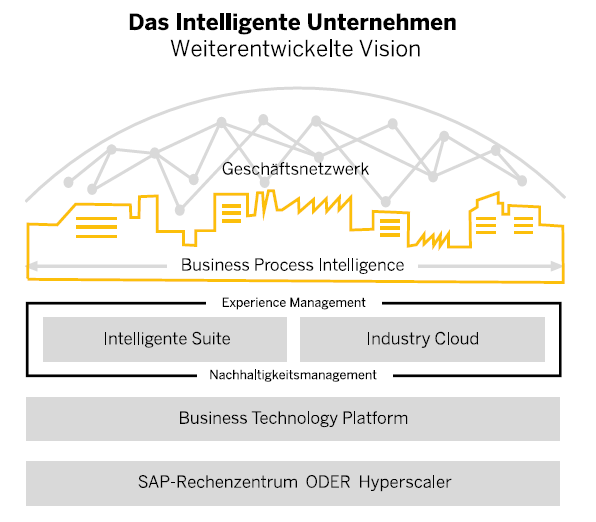
\includegraphics[scale=1]{Bilder/SAPIntelligentesUnternehmen.png}
    \caption[Das Intelligente Unternehmen]{Das Intelligente Unternehmen (\cite[][S. 53]{sap2020-report})}
\end{figure}

Die SAP verfolgt derzeit die Vision ihre Kunden zu einem intelligenten Unternehmen zu entwickeln, in denen die Prinzipien der Innovation, Integration, Agilität und Geschwindigkeit an vorderster Stelle stehen. Außerdem alle Elemente eines Unternehmens verbunden werden und ineinandergreifen. Die Komponenten eines solchen intelligenten Unternehmens sind nach Vorstellungen der SAP ein Geschäftsnetzwerk, das die unternehmensübegreifenden Prozesse miteinander verknüpft, eine Business Process Intelligence, die die Geschäftsprozesse analysiert und optimiert, das Experience Management, das die Daten der Anwender, Kunden und Mitarbeiter analysiert, eine Business Technology Platform, die das Fundament für die Integration und Erweiterung von Anwendungen liefert und dem Kunden Möglichkeiten für künstliche Intelligenz, maschinelles Lernen und Prozessautomatisierung bietet, und einem SAP-Rechenzentrum oder einem Hyperscaler, also einem Infrastrucute-as-a-Service Anbieter wie Amazons AWS oder Microsoft Azure.\footcite[Vgl.][S. 53 f.]{sap2020-report}. Dadurch soll das Ziel erreicht werden, langrfritistig die Abläufe der weltweiten Wirtschaft zu verbessern.


\subsubsection{SAP-ERP}
SAP ERP, oder auch SAP ECC (SAP ERP Central Component), ist die Weiterentwicklung der dritten Generation des SAP ERP-Systems, \glqq{}SAP R/3\grqq{}, das im Jahr 1992 die zweite Produktgeneration \glqq{}SAP R/2\grqq{} ablöste und im Jahr 2003 in \glqq{}SAP ERP\grqq{} umbenannt wurde.\footcite[Vgl.][]{sap-unterschiede} Der Name setzt sich dabei aus dem \glqq{}R\grqq{} für den Begriff \glqq{}Realtime\grqq{}, also Echtzeit, für die Echtzeitdatenverarbeitung und der \glqq{}3\grqq{} zum einen für die dritte Generation, aber auch für die dreischichtigen Architektur, die dem System zugrunde liegt, bestehend aus Datenbank, Anwendungsserver und Client. Die dritte SAP-Generation verfügt dabei über eine zentrale Datenbank, in der alle Daten aus den einzelnen Modulen und den verteilten Anwendungen gesichert werden. SAP ERP bzw. SAP ECC stellt die Zentrale Komponente der \glqq{}SAP Business Suite\grqq{} dar, in der noch andere Produkte von SAP erhältlich sind, die auf andere Anwendungsbereiche als ERP abzielen, aber mit den selben Daten arbeiten, zum Beispiel dem CRM (Customer Relationship Management) oder dem SCM (Supply Chain Management).\footcite[Vgl.][]{mindsquare-sap} Durch die unterschiedlich ausgerichteten Systeme können sich die Kunden ihre Systemlandschaft frei zusammenstellen und diese spezifisch an ihr Geschäftsmodell anpassen. Dadurch wird eine noch tiefer gehende Integration von Geschäftsprozessen ermöglicht, da all diese Systeme mit der selben, zentrale Datenbanken arbeiten. Die aktuellste SAP-ERP Version ist das Enhancementpackage 8 für SAP ERP 6.0 und ist im Jahr 2016 erschienen, da \glqq{}SAP R/3\grqq{} seit 2015 durch die neuste Generation \glqq{}SAP S/4HANA\grqq{} abgelöst wurde.\footcite[Vgl.][]{sap-version}\\ SAP bietet für das Grundsystem unterschiedliche Modulen an, die das System erweitern und ebenfalls durch die Kunden frei, nach ihren jeweiligen Anforderungen, zusammengestellt werden können.

\begin{figure}[h]
    \centering
    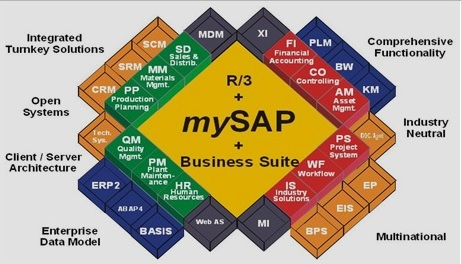
\includegraphics[scale=1]{Bilder/sap-module.jpg}
    \caption[Die Module von SAP-ERP]{Die für SAP-ERP erhätlichen Module (\cite[][]{sap-module})}
    \label{fig:sapmodule}
\end{figure}

In der Abbildung \ref{fig:sapmodule} sind die für SAP-ERP erhältlichen Module und die dazugehörigen Anwendungen bzw. Systeme abgebildet. Die wichtigsten Module und gleichzeitig den Kern des Systems stellen dabei die Module FI, CO, MM, SD, PP und HCM dar, die zum Teil auch standardmäßig in jeder SAP-Installation vorinstalliert sind.\footcite[Vgl.][S. 8]{sap-für-wp} Auf der rechten Seite der Abbildung \ref{fig:sapmodule} sind im inneren Kreis der äußeren Umrandung der Raute, in rot, die Module des Rechnungswesen dargestellt, FI für das externe Rechnungswesen und CO für das Controlling, bzw. das interne Rechnungswesen sind dabei am weitesten verbreitet. Auf der linken Seite sind in grün die Logistikmodule zu sehen, bei denen PP für die Produktion, MM für die Materialwirtschaft, SD für den Vertrieb und PM für die Instandhaltung im Vordergrund stehen. Als dritte Kategorie kommt in den aktuellen Versionen von SAP ERP noch das Modul Human Capital Management (HCM) für die Personalwirtschaft dazu, das das HR-Modul abgelöst hat.\footcite[Vgl.][]{sap-module2} Im äußeren Kreis der äußeren Umrandung der Raute sind in blau die Module der SAP Business Suite dargestellt und in orange die zusätzlich erhältlichen SAP-Produkte, für CRM, SCM, etc.\footcite[Vgl.][]{sap-module}

\subsubsection{SAP HANA}
SAP HANA ist eine sogenannte "In-Memory"-Datenbanktechnologie, die eigens durch die SAP für ihre Produkte entwickelt wurde, mit der große Datenmengen schnell ausgewertet werden können. Die Abkürzung HANA steht dabei für \glqq{}Hyper Perfomance Analytic Appliance\grqq{}, zu deutsch etwa \glqq{}Höchstleistungsauswertungsinstrument\grqq{}. Die Technologie wurde bereits im Jahr 2008 von SAP in Zusammenarbeit mit der Universität Stanford und dem Hasso-Plattner-Institut\footnote{Hasso Plattner ist einer der Mitbegründer der SAP} entwickelt. Die Besonderheit von HANA ist, dass es sich dabei um sogenannte \glqq{}In-Memory-Datenbanken\grqq{} und die Inhalte der Datenbank durchgehend im Hauptsspeicher (RAM) geladen sind und nicht, wie bei herkömmlichen relationalen Datenbanken, nur der aktuell für die Verarbeitung benötigte Teil vom Dauerspeicher in den Hauptspeicher geladen wird.\footcite[Vgl.][]{was-hana} Dadurch sollen die Zugriffsgeschwindigkeiten bis \glqq{}[...] zu 100.000-mal schneller als bei einer Festplatte[..]\grqq{}\footcite[Vgl.][]{rz10-hana} sein. Das vollständige Laden der Datenbank bewirkt zwar, dass dadurch der Hauptspeicher stark belastet wird und durch die Datenmengen entsprechend viel Kapazität benötigt, jedoch bewirkt das Moore'sche Gesetz, dass durch das Voranschreiten der Technologien alle 18-24 Monate die mögliche Computerleistung verdoppelt wird und gleichzeitig die Preise je Speichereinheit sinken.\footcite[Vgl.][]{mooresches}\\ Da, im Gegensatz zu dem stückweisen Laden aus dem Datenspeicher, der Zugriff aus dem Hauptspeicher deutlich schneller von statten geht, ermöglicht HANA somit eine verbesserte Verarbeitung von großen Datenmengen mit hoher Geschwindigkeit. So ist es Unternehmen möglich die gesamte Datenbank in Echtzeit zu analysieren und darauf basierende Entscheidungen zu treffen, wodurch Geschäftsprozess beschleunigt und effizienter gemacht werden können. Eine weitere Besonderheit von HANA ist die Spaltenorientierung, da traditionelle, relationale, Datenbanken in der Regel zeilenorientiert arbeiten und die einzelnen Datensätze je Zeile gespeichert werden. Dadurch ist es möglich, zum Beispiel bei Auswertungen, schnell auf alle Dateneinträge eines Datenbankattributs zuzugreifen, da diese zusammen in einer Zeile gespeichert werden. Auch sind in HANA analytische und transaktionale Daten gemeinsam verfügbar und die analytischen Daten werden nicht, wie bei herkömmlichen Datenbanken, vorher repliziert. Dadurch arbeiten Analysen in HANA stets mit den aktuellen, transaktionalen, Datensätzen. Um die Schreibvorgänge zu beschleunigen, gibt es in HANA einen Buffer, der die zeilenbasiert gelieferte Daten in die benötigte Spaltenstruktur umwandelt.\footcite[Vgl.][]{was-hana}\\Ein Problem, das bei In-Memory-Datenbanken besteht, ist die Erfüllung der sogenannten ACID-Kriterien, die von Datenbanken, bzw. Datenbank-Managementsystemen erfüllt werden müssen. Das Akronym \glqq{}ACID\grqq{} steht dabei für die Eigenschaften \underline{A}tomicity (Atomarität), \underline{C}onsistency (Konsistenz), \underline{I}solation (Abgrenzung) und \underline{D}urability (Dauerhaftigkeit). Von Natur aus kann die Anforderung der Dauerhaftigkeit bei der Datenhaltung im Hauptspeicher nicht gegeben werden, da dieser flüchtig ist und im Falle einer Stromunterbrechung durch einen Stromausfall, oder Systemabsturz seine Daten verliert. Um dieses Problem zu lösen gibt es in HANA einen \glqq{}Persistenz Layer\grqq{}, der dafür sorgt, das die Datenbank in regelmäßigen Abständen (standardmäßig 300 Sekunden) in Form von \glqq{}Savepoints\grqq{} (Sicherheitspunkten) auf einem Dauerspeicher gesichert wird. Um auch nichtbeendete Transaktionen auf der Datenbank wiederherzustellen, gibt es die Möglichkeiten den letzten Zustand anhand von Logs zu rekonstruieren. Auf dem selben Weg ist es auch möglich den vorherigen Zustand nach Abbruch einer Datenbanktransaktion wiederherzustellen, wodurch zugleich auch die Eigenschaft der Konsistenz gewährleistet wird.\footcite[Vgl.][]{rz10-acid}

\subsubsection{SAP S/4HANA} 
SAP S/4HANA ist die neuste Generation 

\subsection{Transformation}
\subsubsection{Definition}
Unter einer Transformation versteht man im allgemeinen einen grundlegenden Wandel, der durch bestimmte Faktoren, wie z.B. einer sprunghafte wirtschaftlichen, oder technologischen Entwicklung hervorgerufen wird. Die Transformation hält dabei idR. über einen längeren Zeitraum an und ist erst beendet, sobald sich die neu geschaffenen Strukturen etabliert und gefestigt haben.\footcite[Vgl.][]{difu}\\ Im betriebswirtschaftlichen Kontext versteht man unter einer Transformation (oder auch Business Transformation) die gezielte Umgestaltung eines Unternehmens und seiner Geschäftsprozesse, um auf veränderte Bedingungen am Markt einzugehen und sich ihnen anzupassen. Dabei ist das Ziel durch effizientere und vereinfachte Geschäftsprozesse einen Mehrwert in Form von niedrigeren Kosten bei gleichbleibender, oder bestenfalls verbesserter Qualität zu erreichen und dabei zusätzlich die Kundenzufriedenheit zu steigern.\footcite[Vgl.][]{leanix}

\subsubsection{Die vier R der Transformation}
In den 1990er-Jahren wurde durch Gouillart und Kelly das Modell der \glqq{}Vier R der Transformation\grqq{} \footcite[Vgl.][]{4r-modell} entwickelt, was eine mögliche Form der Business Transformation darstellen soll. Aus diesem Modell hat die Beratungsgesellschaft Gemini Consulting (später in der Capgemini SE aufgegangen)\footcite[Vgl.][]{gemini-died} ein Produkt entwickelt, indem die vier R für vier verschiedene Transformationsdimensionen stehen:\\
\begin{figure}[h]
    \centering
    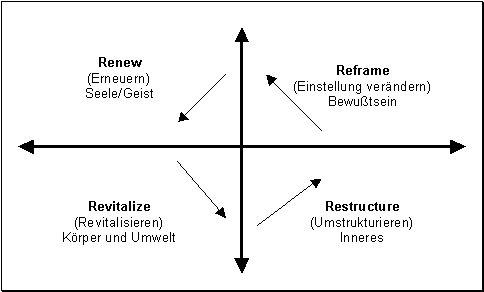
\includegraphics[scale=0.5]{Bilder/businesstransformationManagementportal.png}
    \caption[Die vier R der Transformation]{Die vier R der Transformation (\cite[][]{4r-modell})}
\end{figure}
\begin{itemize}
    \item[] \emph{Reframing (dt. Einstellungsveränderung)} soll in einem Unternehmen dazu beitragen die Sichtweise auf sich selbst zu überdenken um sich dadurch von alten Denkmustern zu befreien. Um diese Einstellungsveränderung anzustoßen ist es wichtig, dass die Mitarbeiter motiviert werden und davon überzeugt sind durch die eingesetze Energie einen Mehrwert zu generieren. Im nächsten Schritt muss anschließend eine Vision definiert werden, die sich erheblich von der präsenten Realität absetzt um im Anschluss daraus Ziele und Messgrößen zu entwickeln. 
    \item[] \emph{Restructuring (dt. Restrukturierung)} 
    \item[] \emph{Revitalising (dt. Wiederbelebung)}
    \item[] \emph{Renewing (dt. Erneuerung)}
\end{itemize}

\subsubsection{Digitale Transformation}
-- Digitale Transformation

\subsection{SAP S/4HANA Transformation}
\subsubsection{Greenfield}
\subsubsection{Brownfield}
\subsubsection{Hybrid}

